\documentclass{gescons}

\genre {Resumo do Biênio}
\author{Amanda Vieira}
\title{Editares celebra 20 anos com programação especial}

\begin{document}
    \makeentrevistatitle
    %\maketitle

    %\fullwidthimage{fields}{b}

    %\coverart{back/editorial}
    \coverart{../fundo-generico.png}
    
    \begin{multicols}{2}

%\begin{center}
%    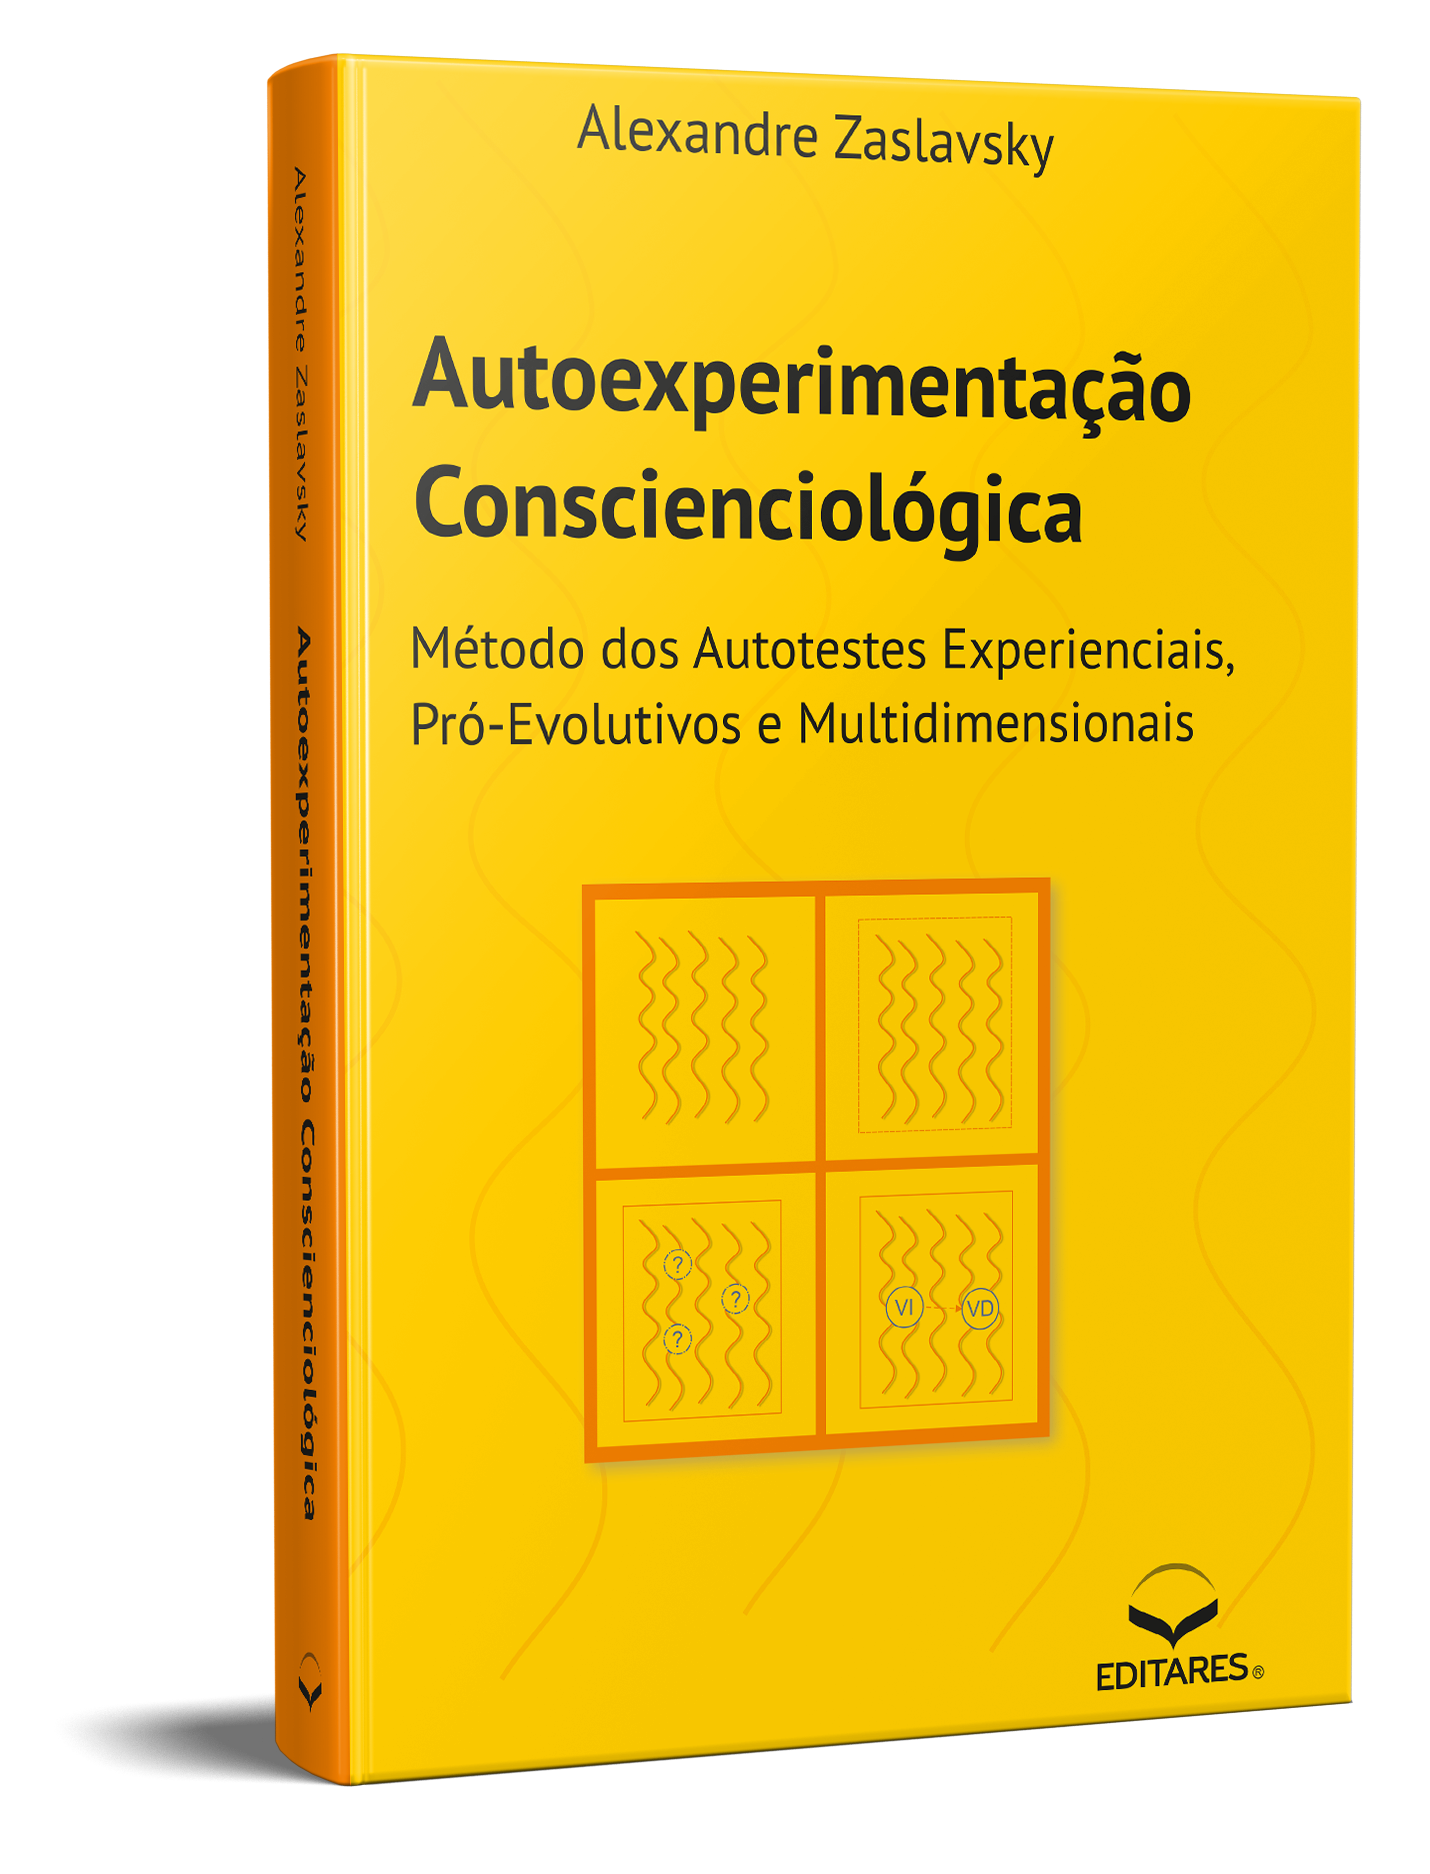
\includegraphics[width=4cm]{articles/entrevista/mockups/Alexandre-Zas.png}
%\end{center}

\textbf{}

\noindent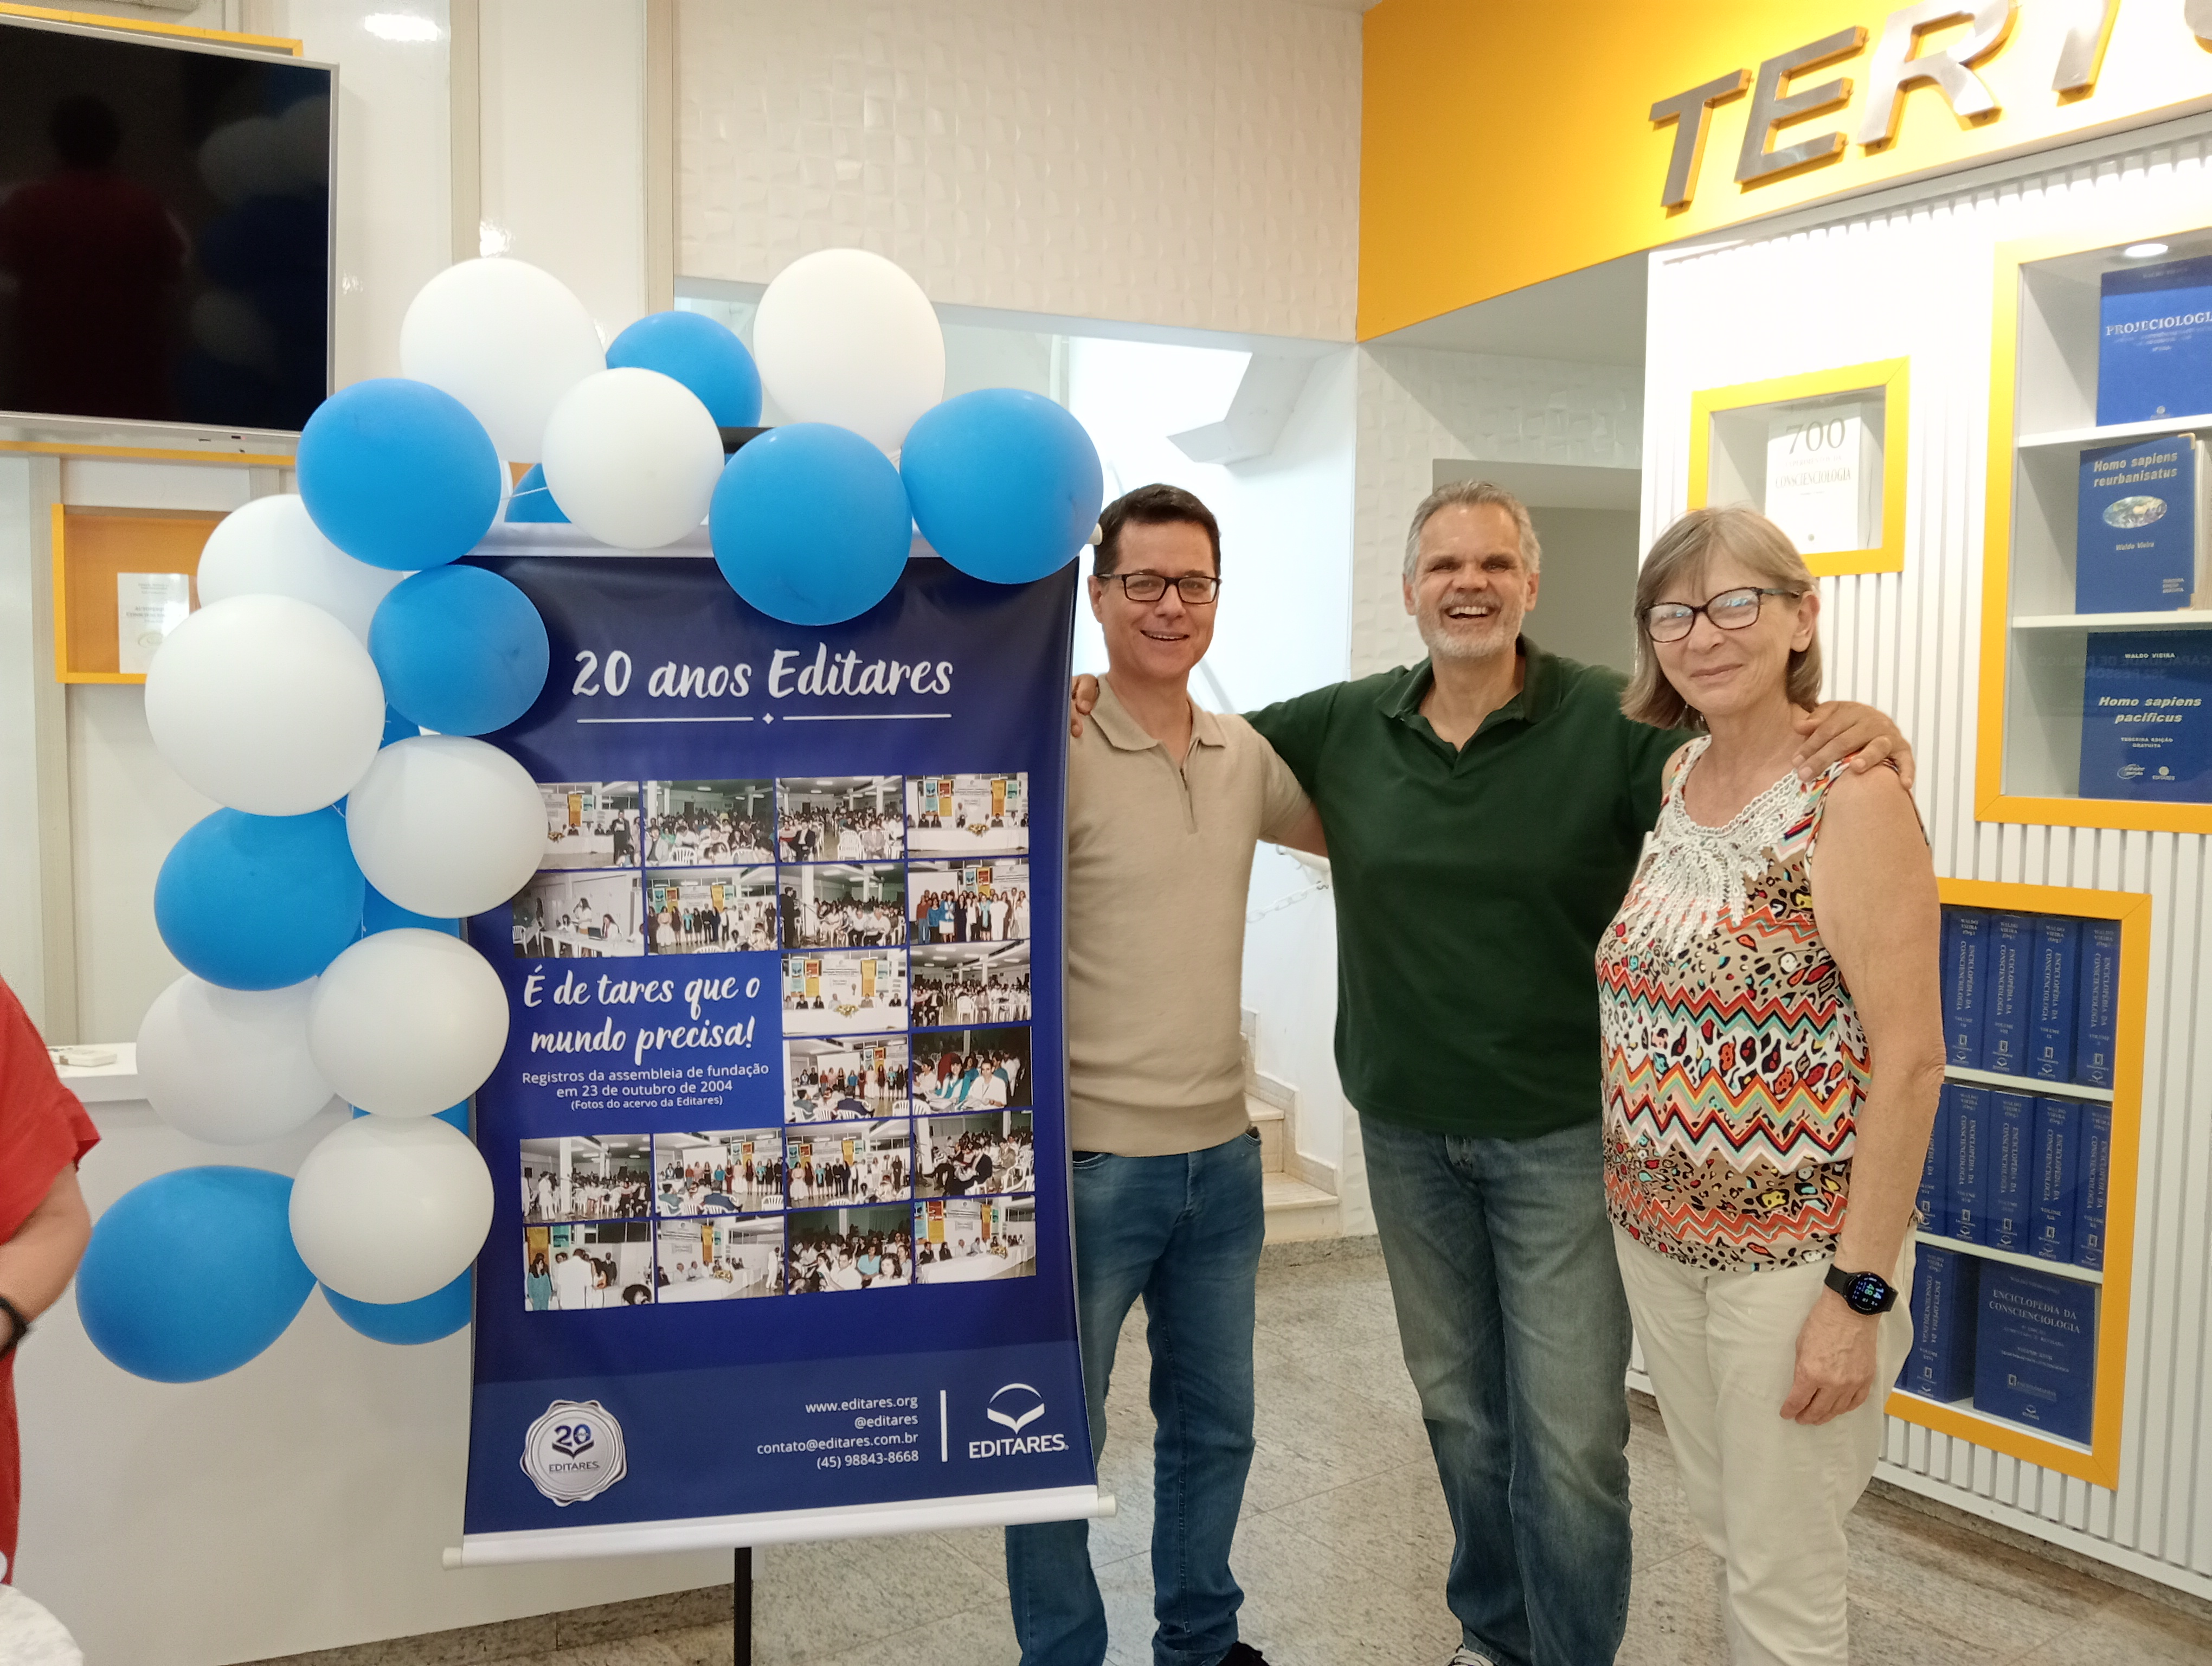
\includegraphics[width=9cm]{articles/resumo/fotos/materia1/IMG20241023144802.jpg}


No dia 23 de outubro de 2024, a Editares completou duas décadas de atuação dedicada à publicação técnico-científica de obras conscienciológicas. Para marcar os 20 anos de existência, a editora promoveu uma série de atividades comemorativas ao longo da semana, integrando voluntários, autores e leitores em momentos de reflexão, confraternização e interassistência.

A programação contou com uma \textbf{semana de verbetes temáticos}, realizada no \emph{Tertuliarium} do CEAEC, com a participação de autores e leitores em debates e apresentações de temas relacionados ao propósito editorial da Editares. Também houve um \textbf{Círculo Mentalsomático temático}, focado na escrita interassistencial e na importância das publicações para a expansão da Conscienciologia.

Um dos pontos altos da celebração foi o \textbf{lançamento do livro ``Interassistência''}, de autoria da voluntária do Conselho Editorial, \textbf{Roberta Bouchardet}. A obra amplia a abordagem da assistência multidimensional.

Além das atividades de debate, os voluntários participaram de um \textbf{jantar temático português}, organizado pelo restaurante Primener, no campus do CEAEC. A noite foi marcada pelo clima de gratidão e união entre os voluntários da Editares e convidados.

No dia 23, data oficial do aniversário, a comemoração seguiu após a Tertúlia, com \textbf{bolo comemorativo e momentos de confraternização} entre voluntários, amigos e apoiadores da Editares, celebrando o continuísmo do trabalho em equipe e o compromisso com a tarefa esclarecedora.

Com 20 anos de história, a Editares reafirma seu papel na difusão da Conscienciologia por meio da escrita e da publicação de obras que promovem o esclarecimento e a evolução das consciências. A celebração reforçou o valor da escrita interassistencial como instrumento de mudança e continuidade da maxiproéxis grupal.

% {[}COLOCAR ALGUMAS FOTOS{]} As fotos estão na pasta do drive: Matéria 1: Editares celebra 20 anos com programação especial - elas podem ser num tamanho pequeno; aparecer no final ou intercalando com o texto

%\begin{pullquote}
%``A escrita de uma obra conscienciológica é uma oportunidade evolutiva inigualável.''
%\end{pullquote}

\noindent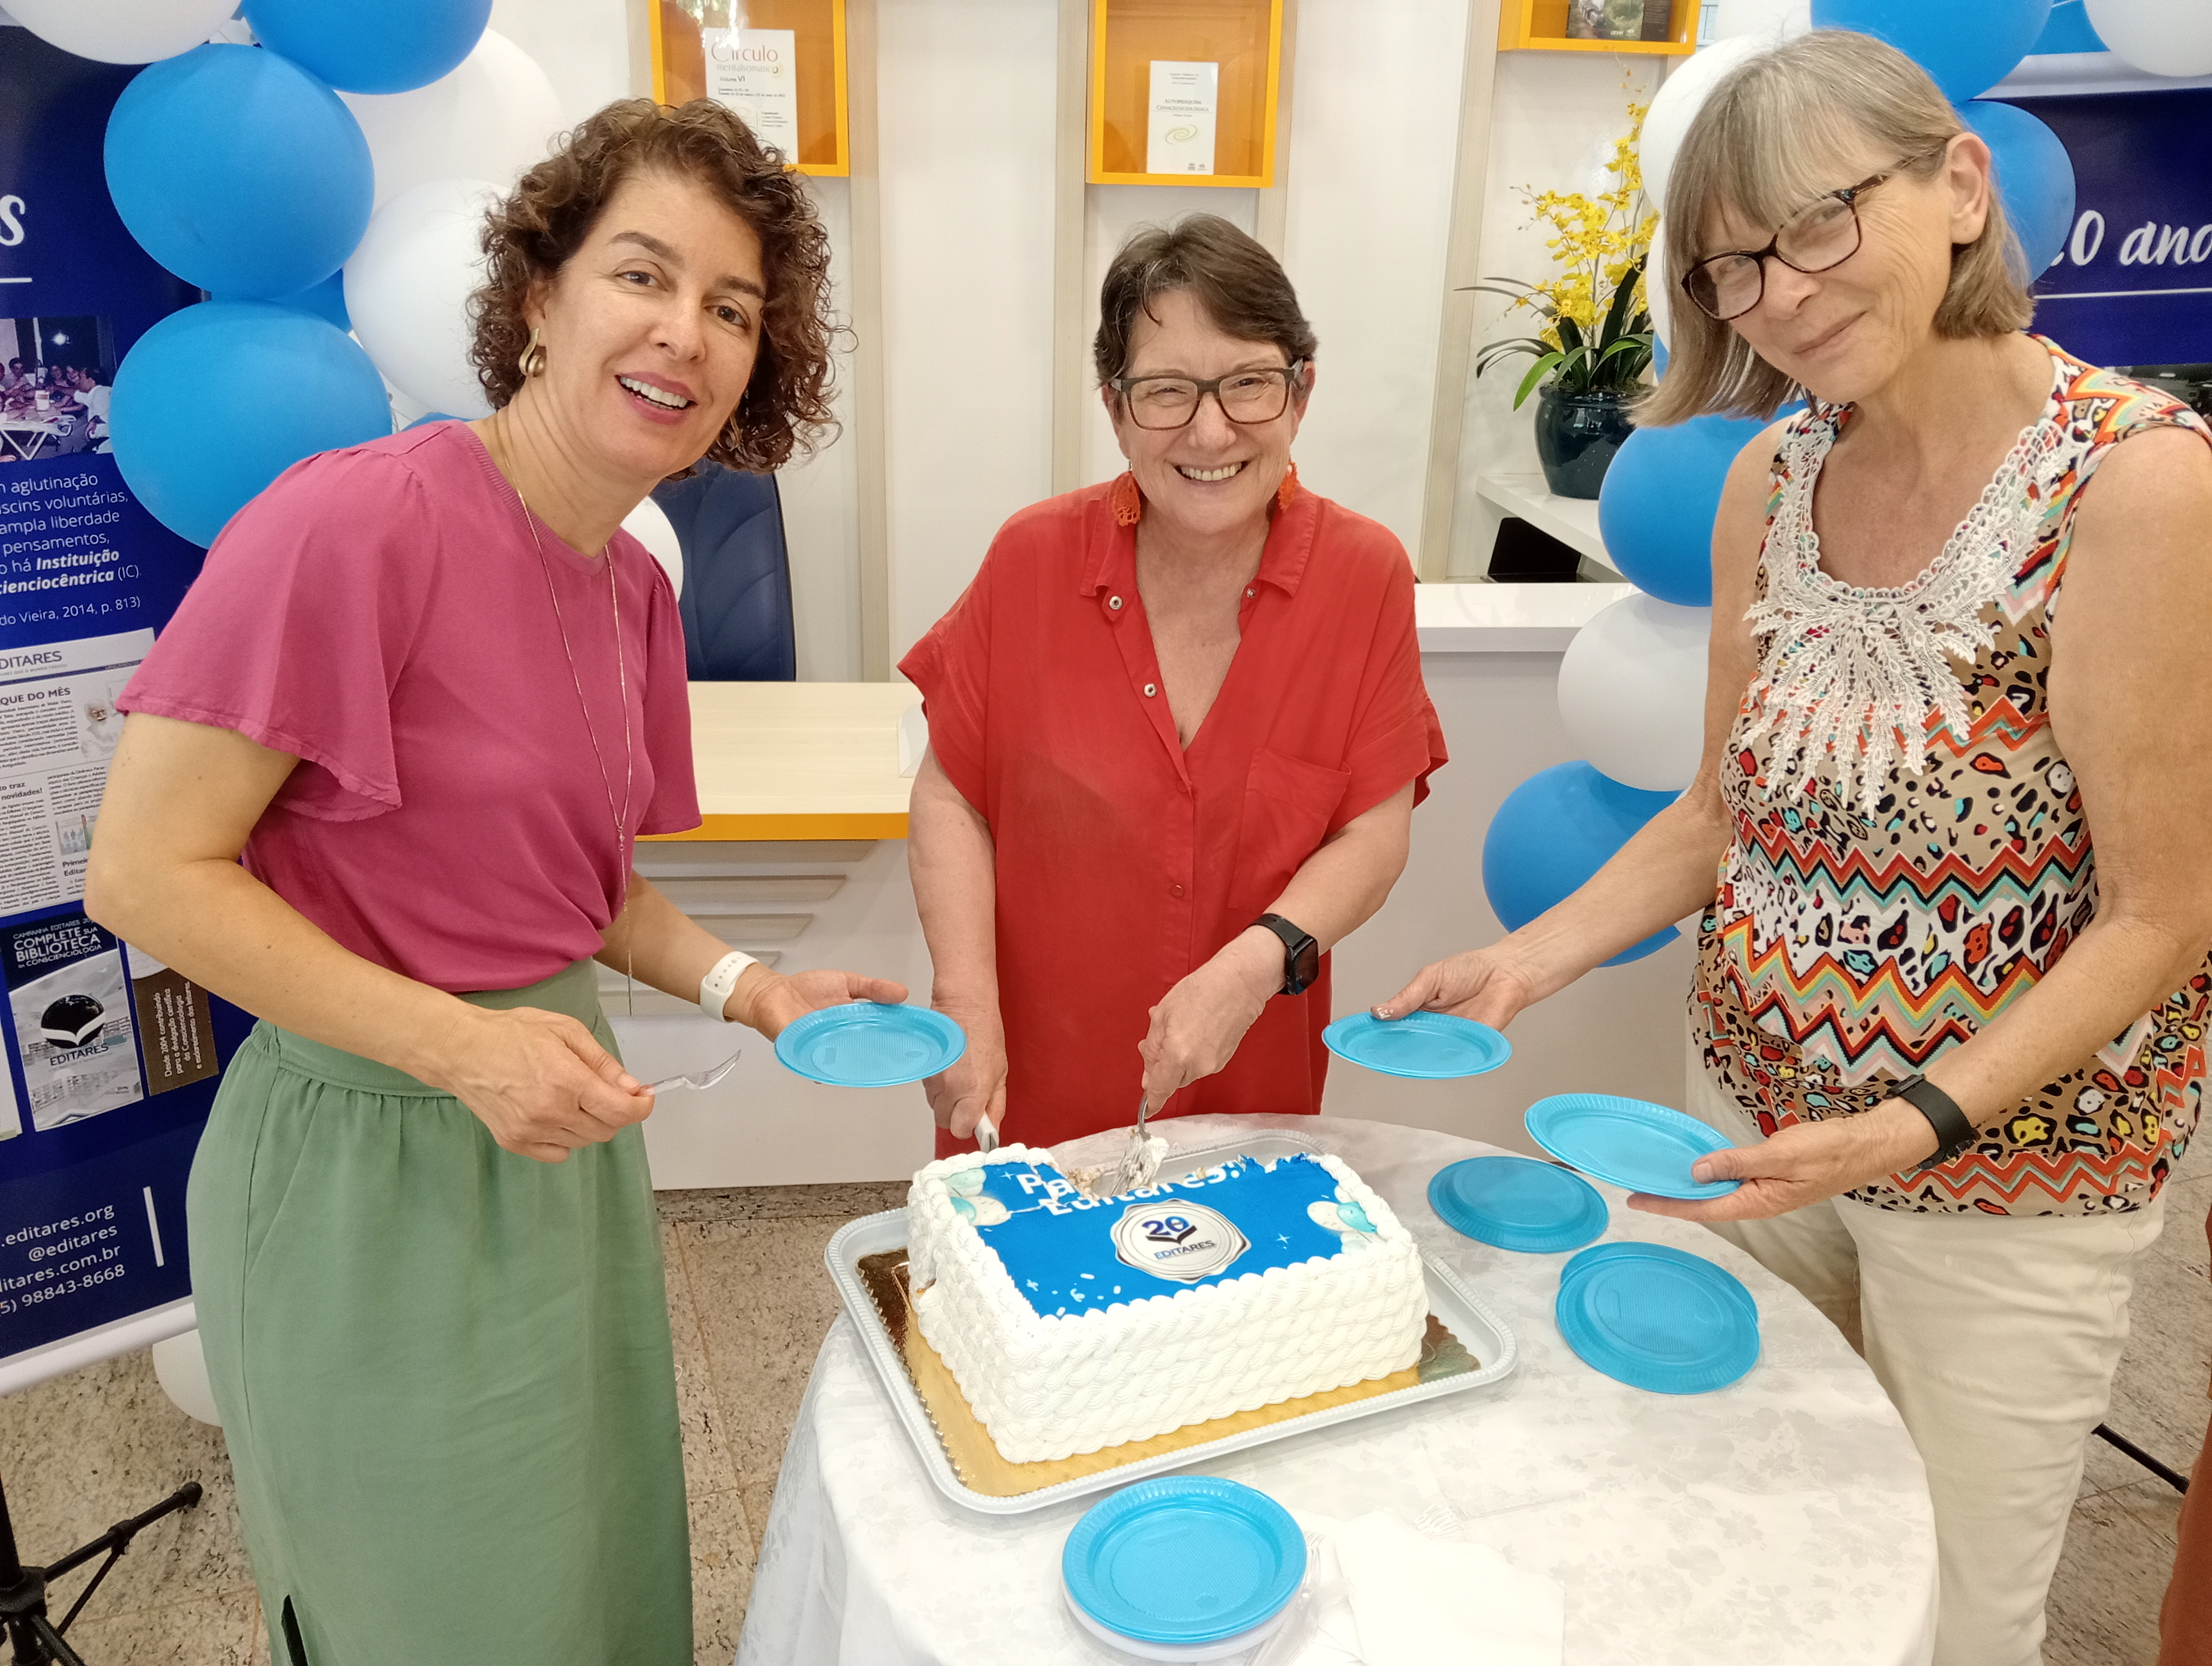
\includegraphics[width=9cm]{articles/resumo/fotos/materia1/IMG20241023143149.jpg}
        
    \end{multicols}
\end{document}
